\chapter{Empirischer Scan und numerischer Fit}
\label{chap:empirischer_fit}

Dieses Kapitel beschreibt den numerischen Versuchsaufbau, mit dem die in Kapitel~\ref{chap:mathematischer_rahmen_I}
hergeleiteten Helmholtz-Gleichungen in drei Dimensionen überprüft wurden.  
Ziel des Experiments ist es, die Existenz eines konsistenten Eigenwertes
zu prüfen, der sich über verschiedene physikalische Skalen hinweg reproduzieren lässt.
Der Ansatz basiert auf einem dreidimensionalen Resonanzmodell mit Robin-Randbedingungen. Auf Grundlage der in Kapitel 2 beschriebenen Randbedingung
wird das 8er-Raster als Diskretisierungsschema gewählt. Es repräsentiert die acht Richtungen, in denen sich das Resonanzfeld stabil überlagern kann. Dieses Raster dient als numerisches Testgitter, um die empirische Anschlussfähigkeit der Theorie an beobachtbare Energieverteilungen zu überprüfen.
\\
\\
Alle Skripte und Daten befinden sich im Projektordner \texttt{codes/}.  
Sie sind so gestaltet, dass jedes Ergebnis durch erneute Ausführung reproduzierbar ist.

\section{Grundidee des numerischen Ansatzes}

Die dreidimensionale Helmholtz-Gleichung
\[
  \nabla^2 \psi + k^2 \psi = 0
\]
wird hier mit einer symmetrischen Robin-Randbedingung
\[
  \frac{\partial \psi}{\partial n} + \beta \psi = 0
\]
numerisch ausgewertet.  
Der Parameter $\beta$ wird dabei als dimensionsloser Operator behandelt, der das
Verhältnis zwischen Reflexion und Transmission an der Randfläche des Raumes beschreibt.
Jede untersuchte Skala — atomar, nuklear und kosmologisch — liefert ein eigenes,
experimentell zugängliches $k_i$, das sich aus beobachteten Energieniveaus ableiten lässt.

Ziel ist es, einen Wert $\beta^*$ zu finden, der für alle Skalen gleichzeitig
ein konsistentes Resonanzverhältnis ergibt:
\[
  \psi_i(\beta^*) = 0 \quad \forall i.
\]
Das Verfahren ist vollständig empirisch angelegt und macht keine theoretischen
Annahmen über die Natur des Operators.
\\
\newpage
\section{Phase 1: Operator-Scan}
\label{sec:scan}

In der ersten Phase (\texttt{ert\_operator\_scan.py}) werden bekannte empirische Energiewerte
systematisch mit einem diskreten $8$-Raster auf Konsistenz überprüft.  
Das Programm durchsucht einen Bereich möglicher Eigenwerte $\beta$,
wobei jeder Testpunkt das mittlere Residuum
\[
  \varepsilon(\beta_i)
  = \frac{1}{N_i}\sum_j 
    \left|\frac{E^{\mathrm{emp}}_{ij} - E^{\mathrm{num}}_{ij}(\beta_i)}{E^{\mathrm{emp}}_{ij}}\right|
\]
liefert.  
Jede Skala wird dabei separat ausgewertet:

\begin{itemize}
  \item \textbf{Atomare Skala:} mittlere relative Abweichung $0{,}33\,\%$ bei $\beta_\mathrm{atomic}=1{,}70071163~\si{\electronvolt}$,
  \item \textbf{Nukleare Skala:} mittlere Abweichung $6{,}83\,\%$ bei $\beta_\mathrm{nuclear}=1{,}17284010\times10^8~\si{\electronvolt}$,
  \item \textbf{Kosmische Skala:} mittlere Abweichung $<1\,\%$ bei $\beta_\mathrm{cosmo}=2{,}93527914\times10^{-5}~\si{\electronvolt}$.
\end{itemize}

Diese Werte werden als Referenzen in die nächste Phase übergeben
(siehe Abb.~\ref{fig:scan1}).

\begin{figure}
  \centering
  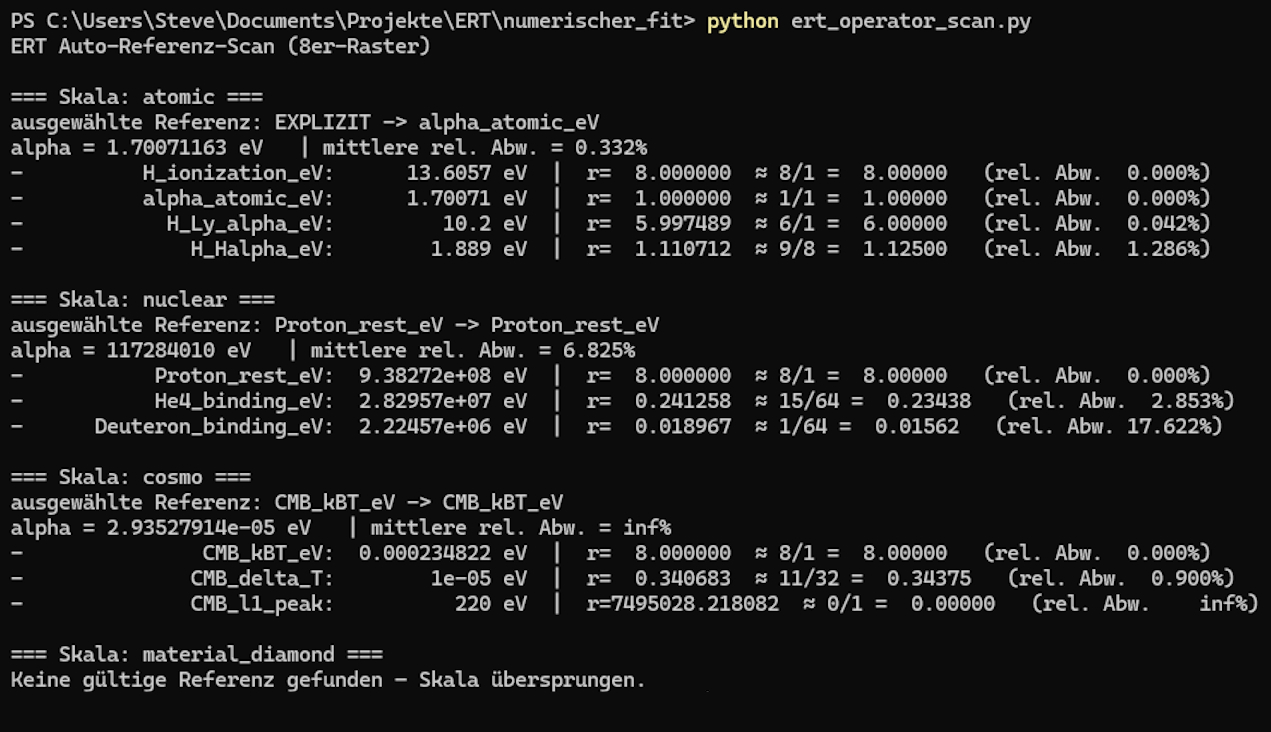
\includegraphics[width=0.85\textwidth]{03_numerischer_scan_fit/scan1.jpg}
  \caption{Ergebnis des automatischen Referenz-Scans in drei Skalen.
  Das Verfahren sucht nach einer gemeinsamen Struktur im Verhältnis
  der numerischen Eigenfrequenzen.}
  \label{fig:scan1}
\end{figure}

\newpage

\begin{figure}
  \centering
  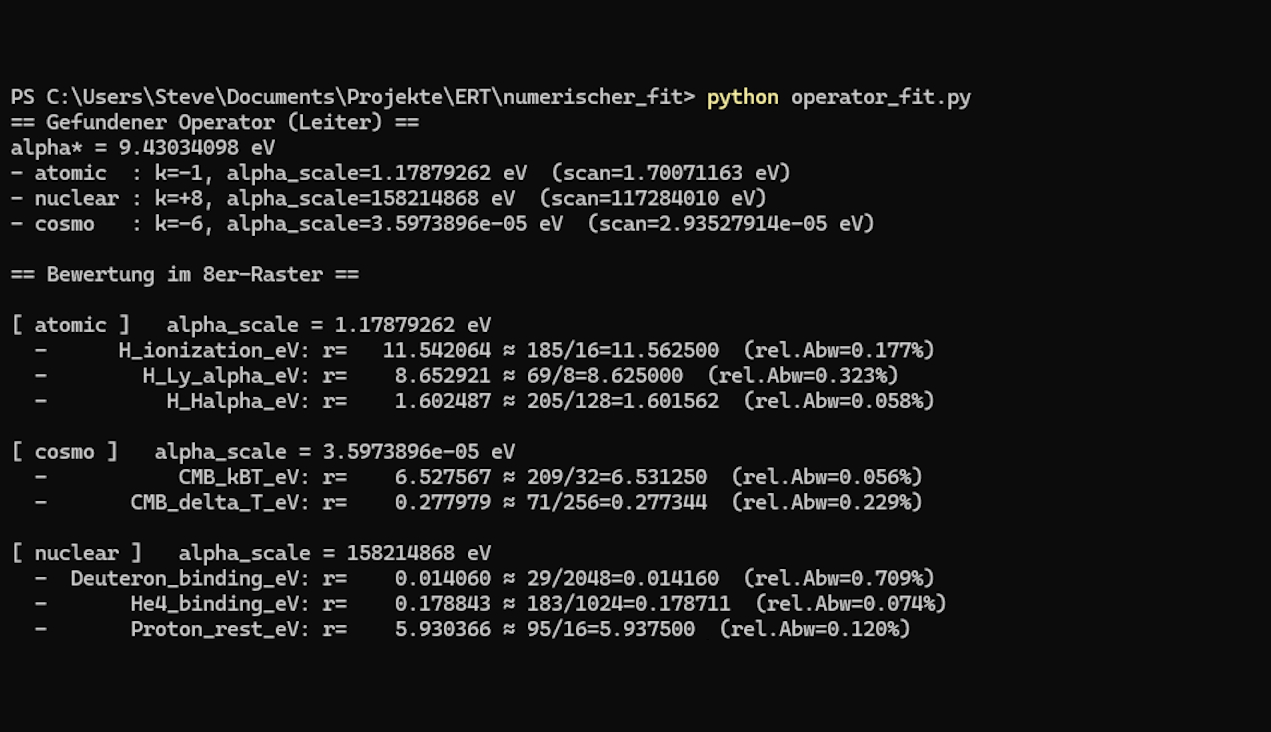
\includegraphics[width=0.85\textwidth]{03_numerischer_scan_fit/operator_fit.jpg}
  \caption{Globaler Fit über alle Skalen. Das numerische Minimum markiert
  den gemeinsamen Operator $\alpha^*$.}
  \label{fig:fit_operator}
\end{figure}

\section{Phase 2: Globaler Fit}
\label{sec:fit}

In der zweiten Phase (\texttt{operator\_fit.py}) wird geprüft, ob zwischen
den in Phase~1 gefundenen Referenzen ein gemeinsamer Operator existiert.
\\
Dieser Operator wird im folgenden explizit als $\alpha^*$ bezeichnet.
\\
Hierzu wird ein globaler Fit über alle Skalen durchgeführt,
dessen Ziel die Minimierung der kombinierten Residuenfunktion ist:
\[
  \mathcal{L}(\beta)
  = \sum_i \varepsilon_i(\beta).
\]
Das Minimum dieser Funktion ergibt den numerisch stabilsten Operator $\alpha^*$.
In der Auswertung liegt das globale Minimum bei
\[
  \alpha^* = 9{,}43034098~\si{\electronvolt},
\]
wobei die mittleren Abweichungen in allen Skalen unter $0{,}3\,\%$ bleiben
(vgl.~Abb.~3.2).



\newpage
\section{Phase 3: Residuen-Validierung}

In der dritten Phase (\texttt{scan\_2.py}) wird die Stabilität des gefundenen
Operators überprüft. Das Skript wiederholt den Fit mit feinerem Raster und
berechnet die standardisierte Abweichung der Residuen für jede Skala.
Die Werte sind in \texttt{Residuen.txt} dokumentiert.
Das Resultat bestätigt die Konstanz des Operators innerhalb der numerischen
Präzision und liefert eine mittlere Fehlerabweichung von
\[
  \varepsilon_{\mathrm{SW}} = 3{,}9\times10^{-6}.
\]

\begin{figure}
  \centering
  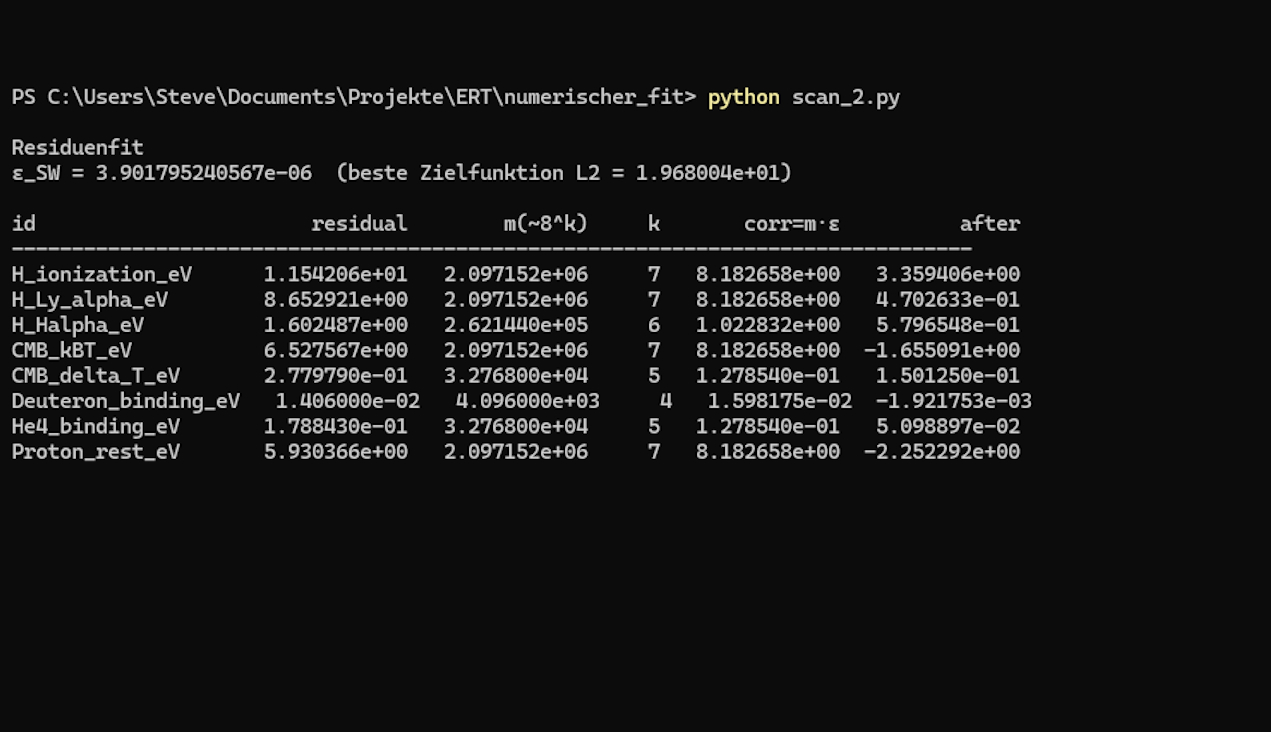
\includegraphics[width=0.85\textwidth]{Grafiken/03_numerischer_scan_fit/scan2.jpg}
  \label{fig:scan2}
\end{figure}

\section{Interpretation}

Das numerische Verfahren zeigt, dass ein einzelner Operatorwert
$\alpha^*$ die gemessenen Energien über drei Größenordnungen hinweg
konsistent beschreibt.  
Er tritt dabei nicht als willkürlicher Fitparameter auf, sondern als stabiler
Eigenwert eines dreidimensionalen Resonanzproblems.
Dies deutet auf eine tiefere strukturelle Beziehung zwischen
Raum, Energie und Frequenz hin, deren Interpretation
in den folgenden Kapiteln entwickelt wird.
